\section{Android app architecture}
The app runs on the users' Android device and was designed to run on Android version 4.0 or greater. As of March 2014 this makes up for 79,7\% of Android devices~\cite{AndroidDeviceFragmentation}. 
The team decided to only adapt the app for these versions because the app is a proof-of-concept, and for the purposes of the app, the team assumed that the relevant users would have a relatively modern phone. 

\subsection{Best practice}

The best practice guidelines for Android~\cite{androidPracticePerformance} states that one should keep the architecture as simple as possible. 
Avoid using large and complex design patterns. But concise code guidelines, and use of tools are needed to keep the development process as simple and effective as possible. 

The app will use a lot of data from a SQlite database, the UI must be responsive, and data will be synchronized from the Internet. To make the app work fluently a good architecture is needed. It is important to note that Android renders the UI on the main thread. Running long operations on the main thread will block the entire app interface. That must be avoided at all cost to not destroy the user experience. 
To avoid the issue of blocking the main thread it was decided to make use of Androids built in logic for async data access, and a design pattern for business logic.

\subsection{Data access}

Data access to the underlying database is done using ContentProviders~\cite{contentproviders}. This gives the app a uniform \gls{CRUD} access model. The data will be accessed with \gls{URI}'s that is uniquely defined. Fetching the data is done using LoaderManager~\cite{loadermanager} . LoaderManager is an interface defining callbacks to get the URI to query, how to handle data reset, and the data returned from the query. The LoaderManager runs on another thread, and thus avoids the problem of halting the UI rendering. It will also handle the life cycle of the data. When data related to the URI changes the the LoaderManager will load the data again. 

ContentProviders contains a lot of boilerplate code and is time consuming to code. But the upsides far outweigh the downsides. When ContentProviders are used with LoaderManager one gets a view that is automatically updated when the data changes without bothering the UI thread. Other solutions are to work directly on the SQLite driver with SQL, or use patters to make it work fluently. But when the choice is between a native building block and a complex pattern the choice is easy to make. 

\subsection{Business logic}

The other problem is related to where to place the business logic for data manipulation. The business logic must be kept in a logic place and not spread around in the view code. That can create hard to find bugs and make it difficult to change how the logic works.
The group decided to use the pattern Model-View-Presenter (MVP). MVP is a Model-View-Controller (MVC) derivative~\cite{mvc}. All business logic is handled in presenter classes, between the views and models. Through this uniform access, all logic applied to data preservation (sever synchronization), and data control can be handled in one place. The life cycle of the presenter classes is in the base Activity class, and all other sub fragments can get access to it though a interface. 
This pushes almost all logic into the presenters, making the code in the fragments as minimal as possible. Since all data is accessed through a ContentProvider it was possible to only adopt this pattern. No view updating code is needed. Only how to manipulate the models and apply it back to the ContentProvider.

\todo{Diagram showing M <-> V <-> P}

\subsection{Server data access}

All data is saved on the server. Communication to server is done with a framework named Volley. It is created by Google and the source code resides within AOSP (Android Open Source Project). It is made to make communication with REST endpoints easier.

Most of all server access is done when synchronizing data with the server~\ref{fig:architecture}. 
Data synchronization is done by using Androids built in SyncAdapter. The SyncAdapter is a self-contained process that that fetches and delivers all new data to and from the server. Communication to the database is done through a ContentProvider. Updating the view is then done automatically of the app is running. 

SyncAdapters can be configured to run when it is suited; It has been a while since last synchronization, there is Internet connection through wifi and the processor is not busy.

\subsection{Keeping the code clean}

Android has a tool named StrictMode~\cite{androidStrictMode}. It can be tweaked to monitors the UI thread and check for file operations, network access and other problems. The penalty for breaking these defined rules can be set to emit a stack trace or kill the app. By having StrictMode configured while coding made discovering bad design easy to detect. 

The app will follow standard Android design guidelines regarding the user interface design.

\todo{class diagram front-end}

\subsection{Patterns}
\subsubsection{Model View Presenter}

\todo{Write about MVP and other patterns that we follow}

\begin{figure}[H]
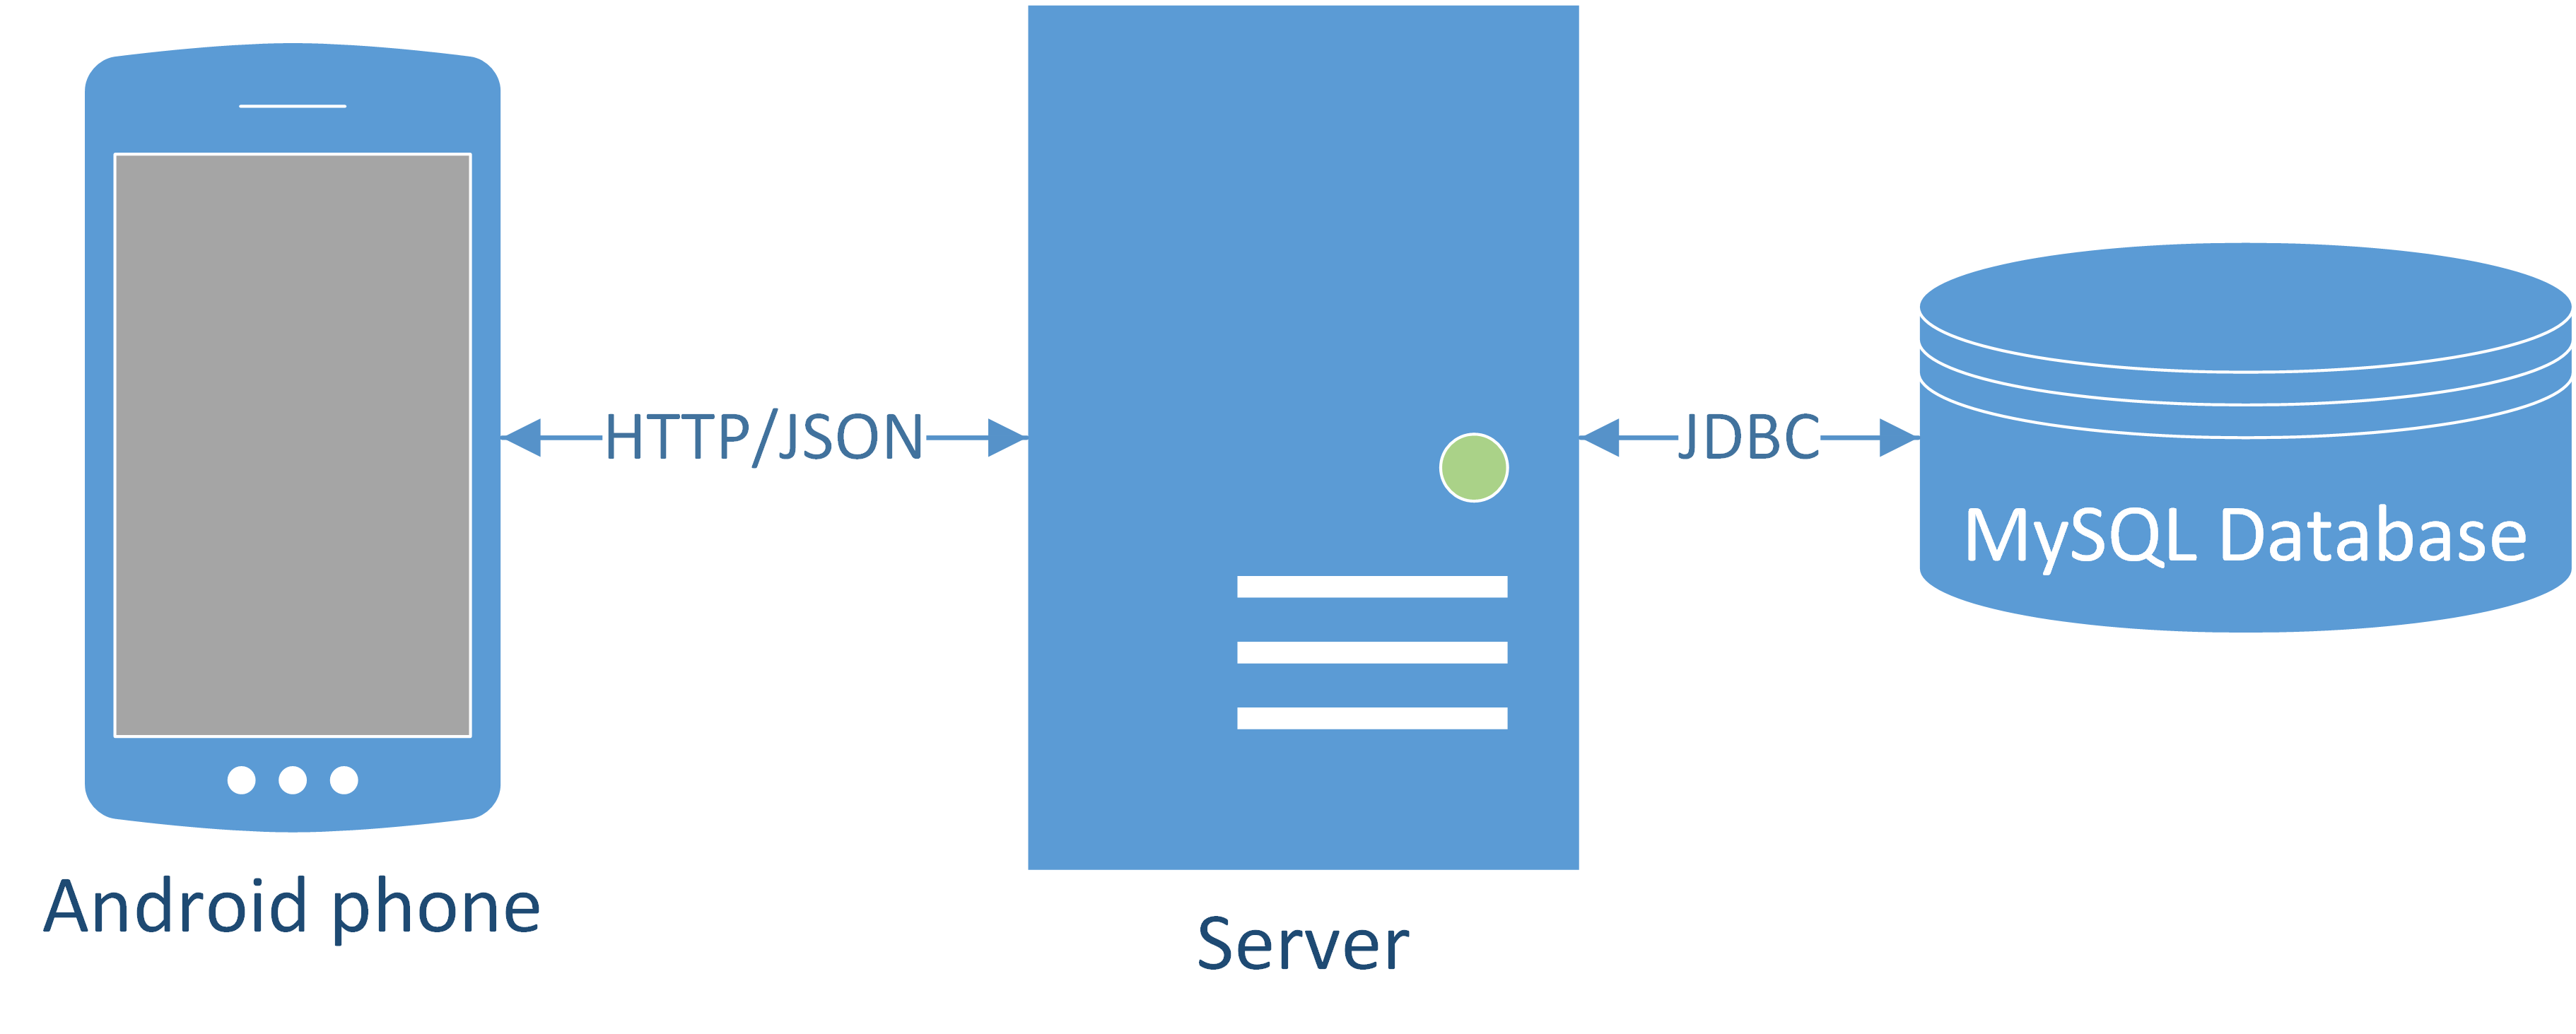
\includegraphics[width=\textwidth]{ch/architecture/fig/arch.png}
\caption{Architecture overview of app communication with the server.}
\label{fig:architecture}
\end{figure}
